In this chapter, we analyze the first experiment group, that is, the impact of using different consensus algorithms on the Blockchain-based Federated Learning system. The consensus algorithms are part of the blockchain itself. Therefore, they do not impact horizontal and vertical FLs differently. In this set of experiments, all properties of the system are static, except for the consensus algorithm, which varies between PoA, PoW and QBFT.

\section{Execution Time, Transaction Cost, and Transaction Latency}

The first performance evaluation metrics we look into are the mean time it takes for a round to complete, the mean transaction latency, and the mean transaction cost. These values are presented in \autoref{tab:metrics_consensus_algorithms}.

\begin{table}[!ht]
\centering
\begin{tabular}{c|c|c|c} \hline \hline
Metric                              & PoA    & PoW    & QBFT   \\ \hline \hline
E2E Time (m)            & 18.93  & 30.62  & 18.97  \\ \hline
Mean Round Time (s)             & 22.70  & 36.72  & 22.74  \\ \hline
% Median Time Per Round (s)           & 21.90  & 35.28  & 21.99  \\ \hline \hline
Mean Transaction Latency (s)    & 1.549  & 1.821  & 1.558  \\ \hline
% Median Latency Per Transaction (s)  & 1.549  & 1.554  & 1.555  \\ \hline \hline
Mean Transaction Cost (Gas)     & 183124 & 227052 & 182880 \\ \hline
% Median Cost Per Transaction (Gas)   & 185198 & 229866 & 185068 \\ \hline \hline
\end{tabular}
\caption{Execution Time, Transaction Cost, and Latency of Consensus Algorithms}
\label{tab:metrics_consensus_algorithms}
\end{table}

Regarding time, we can observe that different consensus algorithms can lead to very different execution times. On the one hand, PoA and QBFT are the fastest consensus algorithms, providing the lowest execution times. Additionally, the difference between both is minimal, i.e., only $0.04$ seconds per round. On the other hand, PoW takes the longest, being $1.6$ times slower than both PoA and QBFT.

Transaction latency and costs follow a similar trend as the execution times. Both PoA and QBFT have similar transaction latency and cost, differing with a small amount, while PoW has a higher transaction latency and cost. PoW costs are $1.2$ times higher than PoA and QBFT.

As explained in \autoref{background:consensus_algorithms}, PoW works by solving increasingly complex mathematical equations that consumes high amounts of resources. This intense process can lead to slower response rates, which translates to higher transaction latency and costs. This, in turn, increases the time it takes for each round to complete.

\section{Model Accuracy and Convergence}

The model accuracy, as well as the convergence, as it can be seen in \autoref{fig:accuracy_consensus_algorithms}, does not change significantly per consensus algorithms. Consensus algorithms determine the order, at which the transactions are processed and ensure consistency between the multiple blockchain nodes. This only affects the blockchain internal processes, and not the ML process. Therefore, it was not expected that the consensus algorithms would have an impact on the model accuracy.

\begin{figure}[!ht]
    \centering
    \centering
    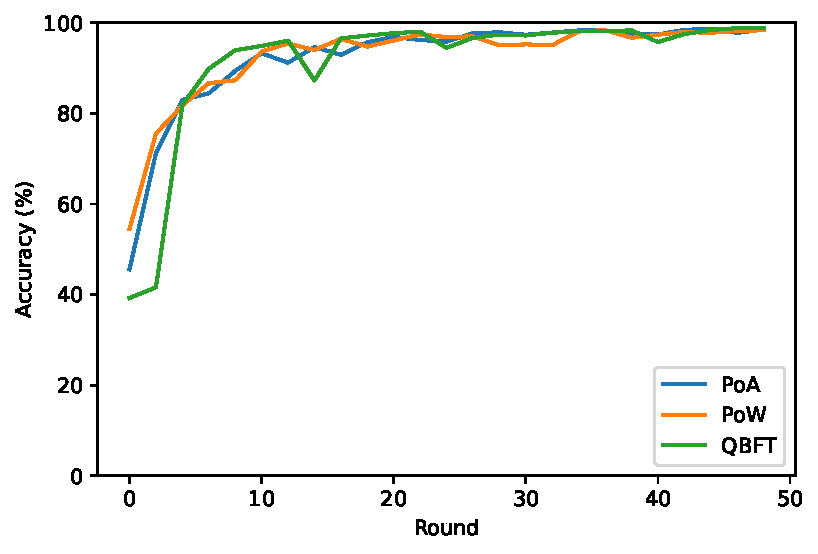
\includegraphics[width=0.7\textwidth]{graphics/consensus/accuracy.pdf}
    \caption{Accuracy Per Consensus Algorithm}
    \label{fig:accuracy_consensus_algorithms}
\end{figure}

\section{Communication Costs}

For the communication costs, we analyze the inbound and outbound network traffic per round at the client, server, and blockchain processes. These values can be observed in \autoref{fig:net_consensus_algorithms}.

On one hand, the inbound and outbound traffic for the clients and server have negligible differences when using different consensus algorithms. As mentioned in the previous section, the consensus algorithms have no expected impact on the ML process. Since the clients and servers only concern the ML process, it was expected that the clients and servers would not be affected. The small differences, in the order of $< 2$ MB, we can observe on the servers are likely related to fluctuations in the random participant selection algorithm. If more participants are being selected, more data needs to be transmitted, and vice-versa. In this case, 17.9, 18.3, and 17.7 clients participated in each round, on average, for PoA, PoW and QBFT, respectively.

On the other hand, the traffic at the blockchain process varies considerably depending on the consensus algorithm used. On average, PoW requires more bandwidth per round than PoA, but the difference is minimal. However, QBFT requires $2$ times more network traffic than PoW and $4$ times more traffic than PoA. QBFT is a three-phase consensus algorithm, which requires a higher number of network messages to be transmitted before reaching a consensus. In addition, the size of the messages also differs. When combining both of these aspects, we can conclude that the expected network traffic per round using the QBFT algorithm would be higher, as verified.

\begin{figure}[!ht]
    \centering
    \centering
    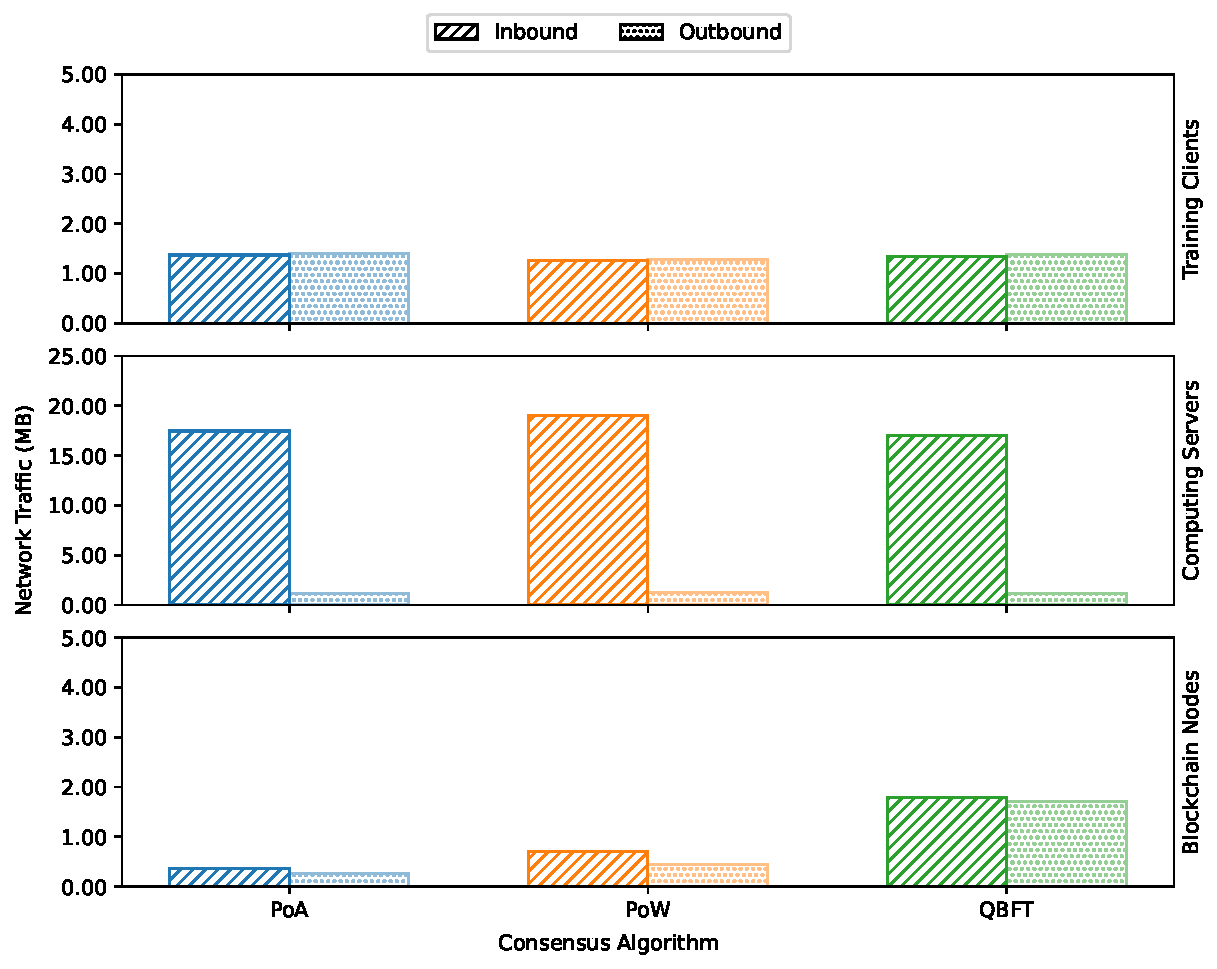
\includegraphics[width=0.8\textwidth]{graphics/consensus/net.pdf}
    \caption{Network Traffic Per Round Per Consensus Algorithm}
    \label{fig:net_consensus_algorithms}
\end{figure}

\section{Computation Costs}

Regarding computation costs, we look at both RAM and CPU usage on the client, server, and blockchain processes. \autoref{fig:ram_consensus_algorithms} and \autoref{fig:cpu_consensus_algorithms} show the mean RAM usage and mean CPU usage, respectively, per consensus algorithm during the execution of the experiments. As mentioned previously, the execution times for PoA and QBFT are lower than for PoW, which can be seen in the figures by not showing more data past minute 19. Additionally, as explained before, the consensus algorithms are not expected to have a direct impact on the clients or the servers.

\begin{figure}[!hpt]
    \centering
    \centering
    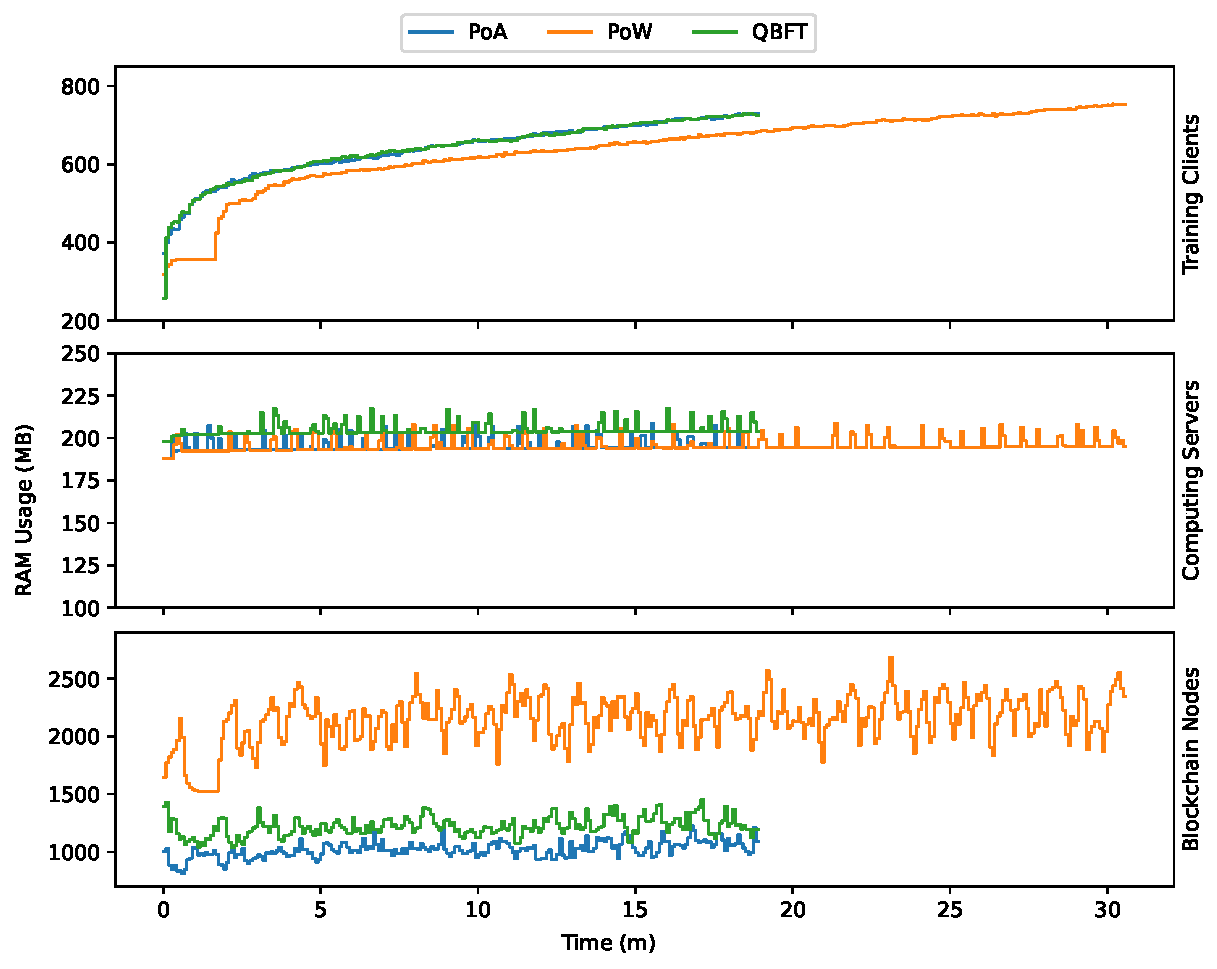
\includegraphics[width=0.8\textwidth]{graphics/consensus/ram.pdf}
    \caption{RAM Usage Per Consensus Algorithm}
    \label{fig:ram_consensus_algorithms}
\end{figure}

\begin{figure}[!hpb]
    \centering
    \centering
    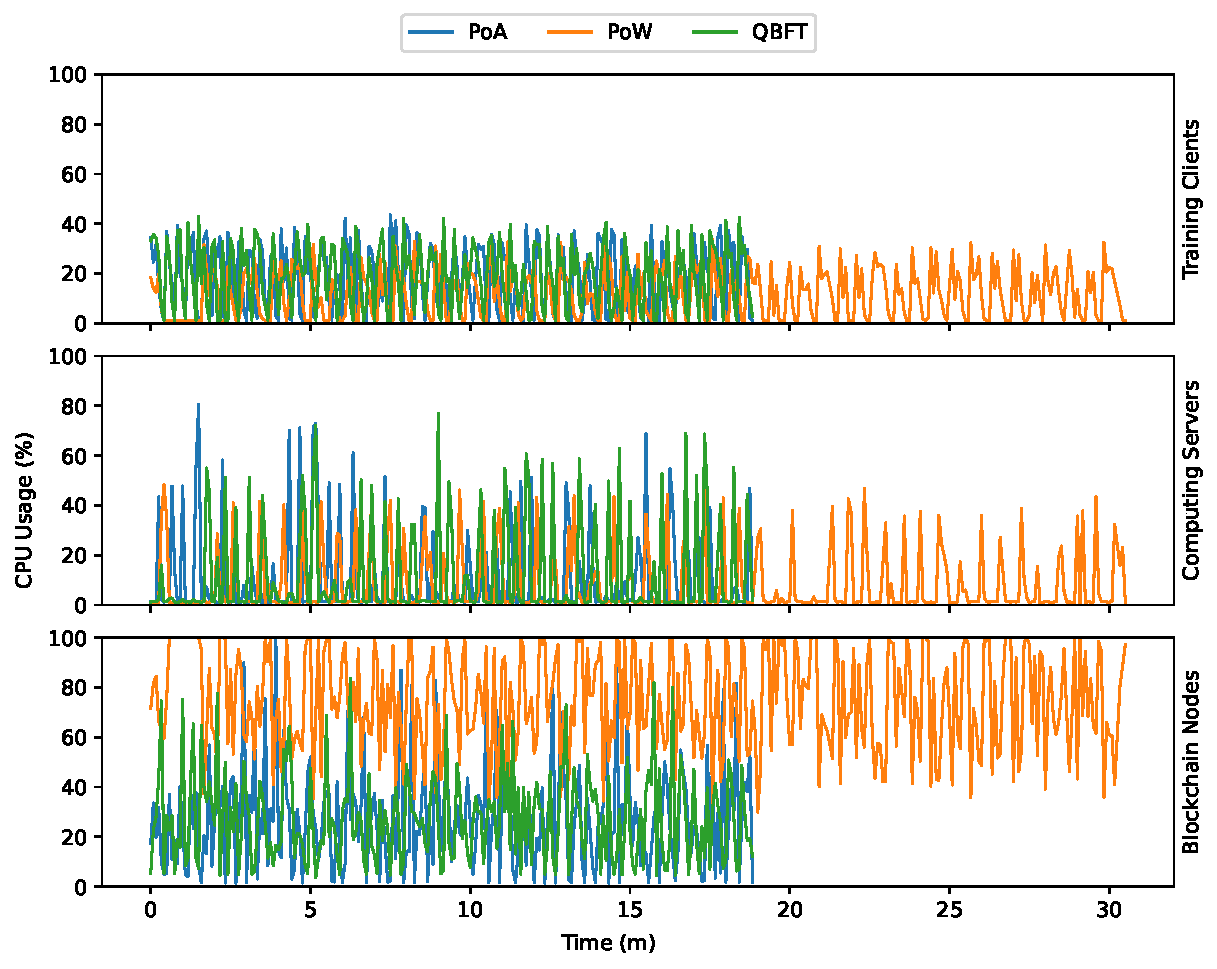
\includegraphics[width=0.8\textwidth]{graphics/consensus/cpu.pdf}
    \caption{CPU Usage Per Consensus Algorithm}
    \label{fig:cpu_consensus_algorithms}
\end{figure}

Regarding the clients, the RAM usage and CPU usage do not differ significantly regardless of which consensus algorithm is used. From the RAM usage, we observe that the clients reach the same peak. However, the rate at which that peak is reached is different. For PoW, since there are higher transaction latencies, it takes longer to reach the next round, leading to a slower growing RAM usage during the model training phase. On the other hand, from the CPU usage, we observe that there are more idle moments, that is, moments at which the CPU usage is lower. This can also be explained by the higher transaction latencies, during which the clients cannot do anything other than wait for the transaction to be approved.

Regarding the servers, the same reasoning as for the clients can be applied. While the RAM usage is consistent across different consensus algorithms, we notice that when using QBFT, the RAM usage at the servers is slightly higher. However, this is a likely negligible difference, as the difference is minimal ($< 10$ MB) considering the total RAM Usage ($\approx 200$ MB). The CPU usage is similar to what we observed for the clients, with a higher amount of idle moments.

Regarding the blockchain process, we observe a larger difference, both in terms of RAM and CPU usages. For both, PoW consumes a much higher level of resources. On average, PoW consumes $2$ times more then RAM and has a $2$ times higher CPU usage. This can also be explained by the way PoW works by solving complex mathematical equations, which require intense computation resources.

\section{Conclusions and Improvements}

In conclusion, we can observe that different consensus algorithms have no direct impact on the model accuracy and computation and communication costs at the clients and servers. However, they have an impact on the time and computation and communication costs at the blockchain process. PoA and QBFT are much faster than PoW. In addition, they require less computation power, both in RAM and CPU. However, QBFT consumes incurs more communication costs than both PoA and PoW. Therefore, there is a clear correlation between the computation costs and the time it takes. The higher the communication costs, the higher the transaction latencies, which translates to slower round times.

Assuming that the blockchain network is only being used for FL, PoA is the most cost-effective of the consensus algorithms we analyzed.

It is also worth pointing out that, as discussed in \Cref{chapter:related_work}, PoA is criticized for not being as decentralized as the other algorithms due to the way the validator nodes are chosen. If a higher degree of decentralization is required, as in a public network for example, PoW and QBFT may be better options. There is therefore a trade-off between the degree of decentralization and the communication and computation consumption.

For future work, it would be interesting to study if the Ethereum blockchain could be adapted to easily incorporate the custom consensus algorithms that were seen in \Cref{related_work:consensus_algorithms}. These algorithms work by producing proofs directly from the Machine Learning process. This can lead to better usage of resources if the blockchain network is solely used for a FL system.